 \newcommand{\figurepath}{./figures/}
\newcommand{\figurescale}{0.5}
\newcommand{\codepath}{../matlab/}


\subsection*{Task 1 and 2}

In task 1 the number of processors where fixed to 4, and different sizes of n where tested. In Fig. \ref{fig:1} the speedup where measured against the size of n in a log scale. For task 2 the speedup where measured against different number of processors and with the problem size fixed to $n=10^6$

\begin{figure}[h!] 
 \center 
 \subfloat[\label{fig:1}]{ 
 \includegraphics[scale=\figurescale]{\figurepath/plot1.eps} } \\
 \subfloat[]{ 
 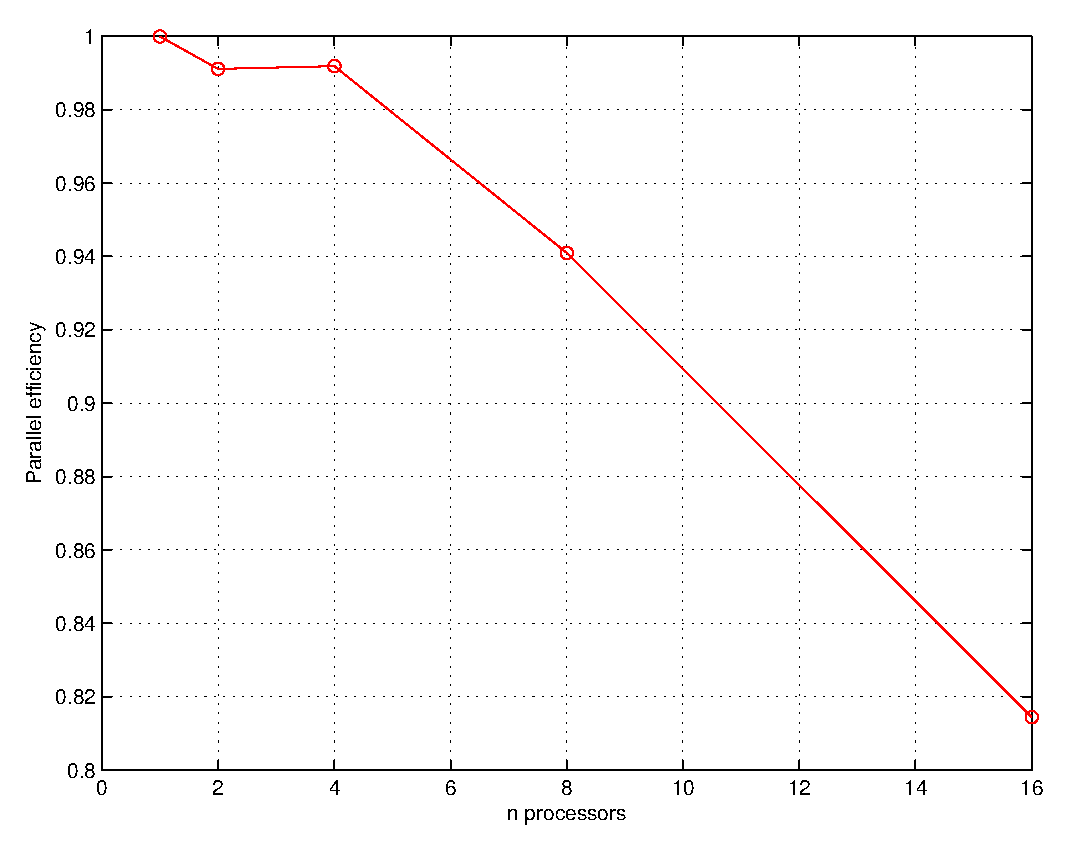
\includegraphics[scale=\figurescale]{\figurepath/plot2.eps} }
 \caption{ Showing a) Speedup for different sizes of n. b) Speedup for different number of processors \label{fig:}}
 \end{figure}


\clearpage

\subsection*{Task 3}

The innerproduct program was tested for $ 20 , 40 , 60, 80, 100, 120, 140 $. The test was run with $n=10^7$ and with $CILK\_NPROCS=8$. From Fig. \ref{fig:co} one can see that for the most part the running time decreases for increasing coarseness. This can be due to the fact that increasing the coarseness leads to a smaller number of spawns, resulting in less overhead.


\begin{figure}[h!] 
 \center 
 \includegraphics[scale=0.6]{\figurepath/plot21.eps}
 \caption{ Plot of running time vs coarsness \label{fig:co}}
 \end{figure}

 

